\section{Q \& A with Temple Layout}

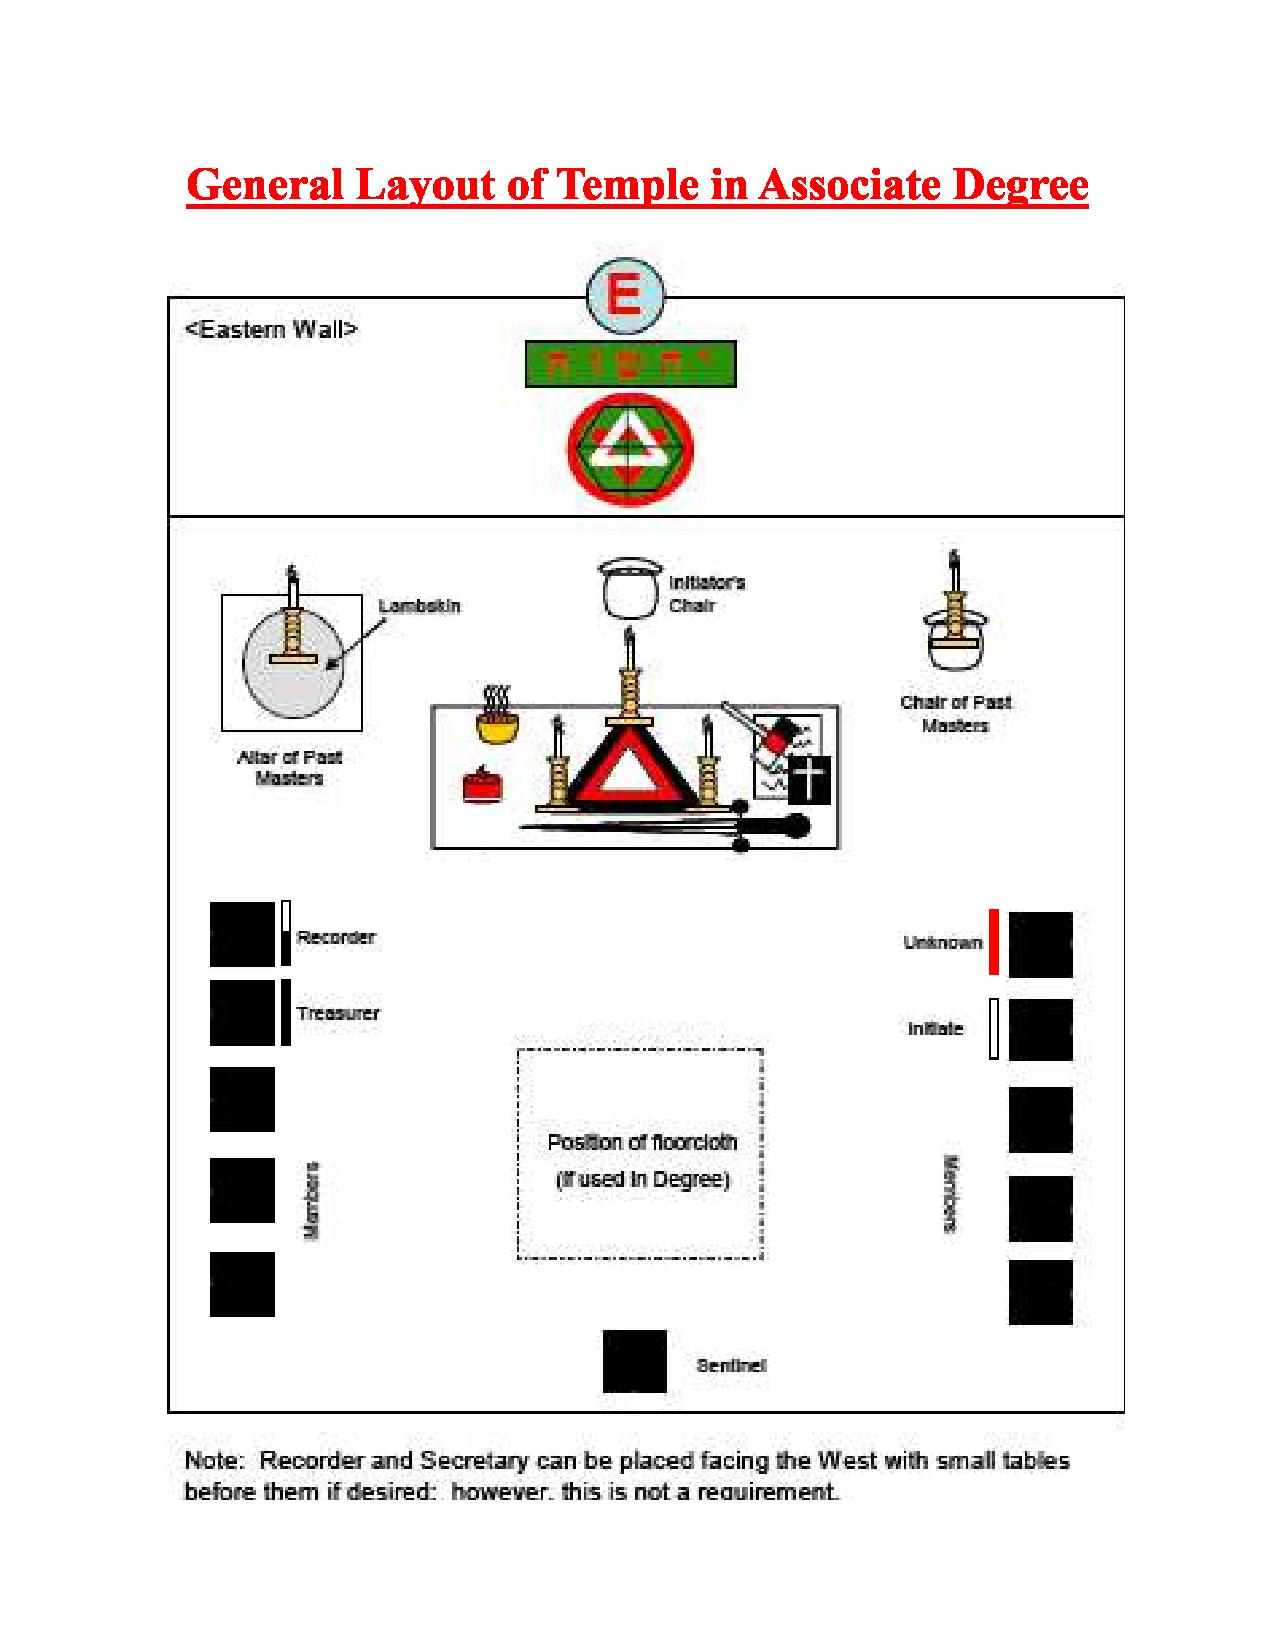
\includepdf[pages=-]{week02/layouts.pdf}

Copying of this material is prohibited without express consent of WM.

\subsection{The Questions \& Answers}

These questions take place between the \textbf{Master Initiate} (MI) and the \textbf{Unknown} (Unk.).

\newcommand{\mi}{\textbf{MI}:}

\newcommand{\unk}{\textbf{Unk.}:}

\mi{}	Are you a Martinist? 

\unk{}	I am a ``Man of Desire'' and aspire to become one. 

\mi{}	What does it mean to be an Associate? 

\unk{}	That the Neophyte has received the Initiation which will permit him/her to take their first steps towards the interior Temple, and that he/she associates him/herself, by his/her own free will, by heart rather than by word, to the common mystical work. 

\mi{}	How many flambeaux are lit for a First Degree Initiation? 

\unk{}	One only, that of the Past Masters. 

\mi{}	Why only this flambeau? 

\unk{}	Because the Neophyte who presents himself/herself to receive the Initiation as Associate is received into the Martinist Order of Unknown Philosophers solely by the Past Masters. 

\mi{}	Where is the Bible placed in this Degree? 

\unk{}	In the First Degree the Bible is placed on the left of the three Luminaries whose flambeau placed in the East represents the Father, that one placed in the North, the Son, and that one in the South, the Holy Spirit. Indeed, with this Degree the Neophyte starts to study the Bible and the Old Testament, written by the Prophets and Inspired people who were under the influence of the Holy Spirit. 

\mi{}	The colour of the Temple in the degree of Associate? 

\unk{}	Blue, because one of the symbolic characteristics of Blue is the abandoning 
of earthly things in order to dedicate oneself to celestial things. 

\mi{}	What is the principal Martinist symbol? 

\unk{}	The Pantacle of the Order, the apex turned to the East. 

\mi{}	What does this Pantacle symbolize? 

\unk{}	It symbolizes the Macrocosm in which the Microcosm must evolve. 

\mi{}	Why is the apex of this Pantacle turned towards East? 

\unk{}	Because the East symbolizes the light. It is also the place where the Sun rises. 

\mi{}	What must be the colour of the groundsheet on which the Pantacle is traced? 

\unk{}	The colour is green to symbolize the Holy Grail, green being the colour of the emerald; and the sacred chalice was made from a great emerald. The legend of the Holy Grail is well known: the Grail was a cup with which Christ celebrated the Last Supper, and in this same chalice Joseph of Arimathea collected the precious blood which flowed from the wounds of our Lord. This cup was made from a single precious stone: a great emerald. Green is the colour of the emerald, and thus the colour of the Grail. It is the colour of Hope; it refers to water, it corresponds to vegetables; it is complementary to red. 

\mi{}	What is the principal part of the Initiation in the degree of Associate? 

\unk{}	The journey beneath the veil where the Neophyte, blindfolded, passes through seven points, including the one he occupies in the centre of the Pantacle. He is led, because his sight is obscured, and yet he searches for the light which alone is in the East. 

\mi{}	Are the teachings of our Order initiatory? 

\unk{}	The teachings of our Order are initiatory, because they are the purest branch of the One and Mother Tradition as it was transmitted from the source through the channel of regular Initiation, up to myself. 

\mi{}	How will you become worthy of the perfect knowledge contained in our symbols and to which Initiation offers the key? 

\unk{}	By my efforts to work with zeal and without respite for the common good of the Order, which is required of every Martinist. By this means shall I attract the benevolence of the Masters, who will unite their works and operations to mine that I might attain to the use of the rights, fruit and prerogatives of the true Martinist. 

\mi{}	My Brother/Sister, the appropriateness of your replies leads me to suppose that you will be able to participate in the united acts of the ``People of Desire.'' I shall ask you a final question: What is the Basis of our Order ? 

\unk{}	The Order serves as a base to the ``People of Desire'' to manifest the teachings through the several ceremonies and so preserve the regularity of the first principles, virtues and spiritual powers. 

\subsection{The Signs \& Words}

The members of our Order have signs and passwords which allow us to 
recognize other Martinists of the Order and to enable us to be recognized by 
them. If you think you are in the presence of a Martinist, here are the 
Questions and Answers to give, which constitute our Signs and Words of Recognition: 

\textbf{Q}: \textit{Pass the first three fingers of the right hand over the right eyebrow. This sign should be made three times, without ostentation.}

\textbf{A}: \textit{Pass the half-closed right hand, three times, behind the right ear.} 

\textbf{Q}: Do you know the path? 

\textbf{A}: I am looking for it. 

\textbf{Q}: Prove it! 

\textbf{A}: \textit{One pressure of the right hand thumb on the first knuckle of the right index of the interrogator.} 

\begin{itemize}

\item \textit{When the Initiator asks you to stand at order, you will give our 
Sign of Order, which is given by putting the right hand open 
wide, flat over the heart.} 

\item \textit{When he/she asks for the Sign, briefly place your index and 
middle fingers across the lips, with the index finger touching 
them.} 

\item The Battery comprises 6 and 1 ($\bullet$\hspace*{1ex}$\bullet$\hspace*{1ex}$\bullet$\hspace*{1ex}$\bullet$\hspace*{1ex}$\bullet$\hspace*{1ex}$\bullet$\hspace*{3ex}$\bullet$) under the direction 
of the Master: six regular beats followed after a short waiting time by the 7th. 

\item To execute the Acclamation each member raises his right hand 
widely open and loudly says the word: Caritas!

\end{itemize}

\subsection{General Points and Reminders}

Once the Temple has been consecrated, there are several protocols which 
must be observed. Here is a list of some of the more important points which you 
should endeavor to learn and exercise:

\begin{itemize}
\item When entering the Temple, give the Acclamation silently by stopping at the 
threshold, coming to Order, and then extending the right hand , open 
widely, to the East, while mentally reciting Caritas. 
\item When leaving the Temple, stop at the threshold, face East, and give the Sign 
by placing the right index and middle fingers across the lips, with the index 
finger touching them. 
\item When moving about the Temple, the direction of movement must ALWAYS 
be clockwise, with the corners being squared. 
\item When addressed by the Worthy Master, stand and briefly come to Order. If 
you are issued a command, acknowledge it by again briefly coming to Order. 
When returning to your seat, also briefly come to Order before sitting. 
When selecting a seat for the Working, keep in mind that whenever 
space allows, Associates and Initiates should sit in the Northern column, 
and SI and above in the Southern. Also, higher ranks or those elder within 
your grade should sit toward the East, with ``younger'' members toward the 
West. 
\item It is the responsibility of the Associate and Initiate members, under the 
direction of the Sentinel and Master Initiate, to set up the Temple that it 
may be consecrated by the SI of the Chapter. This serves the twofold 
purpose of familiarizing the younger members with the layout and 
symbolism of the degree, while allowing the SI to prepare for the deeper 
work to follow. 
\item At the conclusion of the Work, the WM will say ``you may go now.'' At this 
point, Associates and Initiates must depart the Temple, remembering to give 
the Sign when leaving. Once the Temple has been returned to its mundane 
state, you may re-enter to assist with cleaning up. 

\end{itemize}